\newcommand{\nom}{Porte conteneur}
\newcommand{\sequence}{03}
\newcommand{\num}{04}
\newcommand{\type}{TD}
\newcommand{\descrip}{Résolution d'un problème en utilisant des méthodes algorithmiques}
\newcommand{\competences}{Alt-C3: Concevoir un algorithme répondant à un problème précisément posé}
\documentclass[10pt,a4paper]{article}
  \usepackage[french]{babel}
  \usepackage[utf8]{inputenc}
  \usepackage[T1]{fontenc}
  \usepackage{xcolor}
  \usepackage[]{graphicx}
  \usepackage{makeidx}
  \usepackage{textcomp}
  \usepackage{amsmath}
  \usepackage{amssymb}
  \usepackage{stmaryrd}
  \usepackage{fancyhdr}
  \usepackage{lettrine}
  \usepackage{calc}
  \usepackage{boxedminipage}
  \usepackage[french,onelanguage, boxruled,linesnumbered]{algorithm2e}
  \usepackage[colorlinks=false,pdftex]{hyperref}
  \usepackage{minted}
  \usepackage{url}
  \usepackage[locale=FR]{siunitx}
  \usepackage{multicol}
  \usepackage{tikz}
  \makeindex

  %\graphicspath{{../Images/}}

%  \renewcommand\listingscaption{Programme}

  %\renewcommand{\thechapter}{\Alph{chapter}}
  \renewcommand{\thesection}{\Roman{section}}
  %\newcommand{\inter}{\vspace{0.5cm}%
  %\noindent }
  %\newcommand{\unite}{\ \textrm}
  \newcommand{\ud}{\mathrm{d}}
  \newcommand{\vect}{\overrightarrow}
  %\newcommand{\ch}{\mathrm{ch}} % cosinus hyperbolique
  %\newcommand{\sh}{\mathrm{sh}} % sinus hyperbolique

  \textwidth 160mm
  \textheight 250mm
  \hoffset=-1.70cm
  \voffset=-1.5cm
  \parindent=0cm

  \pagestyle{fancy}
  \fancyhead[L]{\bfseries {\large PTSI -- Dorian}}
  \fancyhead[C]{\bfseries{{\type} \no \numero}}
  \fancyhead[R]{\bfseries{\large Informatique}}
  \fancyfoot[C]{\thepage}
  \fancyfoot[L]{\footnotesize R. Costadoat, C. Darreye}
  \fancyfoot[R]{\small \today}
  
  \definecolor{bg}{rgb}{0.9,0.9,0.9}
  
  
  % macro Juliette
  
\usepackage{comment}   
\usepackage{amsthm}  
\theoremstyle{definition}
\newtheorem{exercice}{Exercice}
\newtheorem*{rappel}{Rappel}
\newtheorem*{remark}{Remarque}
\newtheorem*{defn}{Définition}
\newtheorem*{ppe}{Propriété}
\newtheorem{solution}{Solution}

\newcounter{num_quest} \setcounter{num_quest}{0}
\newcounter{num_rep} \setcounter{num_rep}{0}
\newcounter{num_cor} \setcounter{num_cor}{0}

\newcommand{\question}[1]{\refstepcounter{num_quest}\par
~\ \\ \parbox[t][][t]{0.15\linewidth}{\textbf{Question \arabic{num_quest}}}\parbox[t][][t]{0.85\linewidth}{#1\label{q\the\value{num_quest}}}\par
~\ \\}

\newcommand{\reponse}[4][1]
{\noindent
\rule{\linewidth}{.5pt}\\
\textbf{Question\ifthenelse{#1>1}{s}{} \multido{}{#1}{%
\refstepcounter{num_rep}\ref{q\the\value{num_rep}} }:} ~\ \\
\ifdef{\public}{#3 ~\ \\ \feuilleDR{#2}}{#4}
}

\newcommand{\cor}
{\refstepcounter{num_cor}
\noindent
\rule{\linewidth}{.5pt}
\textbf{Question \arabic{num_cor}:} \\
}

%%\usepackage[a4paper]{geometry}
%\geometry{margin={1cm,1.2cm}}
%\usepackage[francais]{babel}
%\usepackage{nopageno} %pas de numérotation de page
%\pagestyle{plain} %numérotation en bas de page, pas d'entête
%\usepackage{hyperref}
%\usepackage[latin1]{inputenc}

%%%%%%%%%%%%%%%%%%%%%%%%%%%%%%%%%%%%%%%%%%%%%%%%%%%%%%%%%%%%%%%%%%%%%%%%%%%%%%%%%%%%%

\usepackage{amsthm}
\usepackage{amscd}
%\usepackage{mathrsfs}
%\usepackage{amsfonts}
%\usepackage[T1]{fontenc}
%\usepackage{theorem}
\usepackage{lscape}
\usepackage{variations}  % pour faire des tableaux de variations
\usepackage{dsfont}
\usepackage{fancyvrb} % pour mettre Verbatim dans une box

% Pour les figures
\usepackage{subfig}
%\usepackage{calc} % Pour pouvoir donner des formules dans les d�finitions de longueur
%\usepackage{graphicx} % Pour inclure des graphiques 
% Attention : pour inclure des .jpg comme dans l'exemple (ou des .png ou .pdf)
% il faut compiler directement en pdf (commande pdflatex).
% Pour inclure des .eps, il faut compiler avec latex + dvips + ps2pdf.
\usepackage{psfrag}
%\usepackage{color}

%%%%%%%%%%%%%%%%%%%%%%%%%%%%%%%%%%%%%%%%%%%%%%%%%%%%%%%%%%%%%%%%%%%%%%%%%%%%%%%%%%%%%

\theoremstyle{definition}
\newtheorem*{thm}{Théorème}
%\theorembodyfont{\rmfamily}
\newtheorem*{defn}{Définition}
\newtheorem{exercice}{Exercice}
\newtheorem*{problem}{Problème}
\newtheorem*{prop}{Proposition}
\newtheorem*{corollaire}{Corollaire}
\newtheorem*{lemme}{Lemme}
\newtheorem*{remark}{Remarque}
\newtheorem*{notation}{Notation}
\newtheorem*{ex}{Exemple}
\newtheorem*{ppe}{Propriété}
\newtheorem*{meth}{Méthode}
\newtheorem*{rappel}{Rappel}
\newtheorem*{voca}{Vocabulaire}
\setlength{\columnseprule}{0.5pt}


%%%%%%%%%%%%%%%%%%%%%%%%%%%%%%%%%%%%%%%%%%%%%%%%%%%%%%%%%%%%%%%%%%%%%%%%%%%%%%%%%%%%%

\newcommand{\bi}{\bigskip}
\newcommand{\dsp}{\displaystyle}
\newcommand{\noi}{\noindent}
\newcommand{\ov}{\overline}
\newcommand{\dsum}{\displaystyle \sum}
\newcommand{\dprod}{\displaystyle \prod}
\newcommand{\dint}{\displaystyle \int}
\newcommand{\dlim}{\displaystyle \lim}

%%%%%%%%%%%%%%%%%%%%%%%%%%%%%%%%%%%%%%%%%%%%%%%%%%%%%%%%%%%%%%%%%%%%%%%%%%%%%%%%%%%%%


%\newcommand{\pgcd}{\mathrm{pgcd}} % pgcd
%\providecommand{\norm}[1]{\lVert#1\rVert} % norme
%\DeclareMathOperator{\Tan}{Tan}  % espace tangent


\newcommand{\N}{\mathbb{N}}
\newcommand{\Z}{\mathbb{Z}}
\newcommand{\Q}{\mathbb{Q}}
\newcommand{\R}{\mathbb{R}}
\newcommand{\C}{\mathbb{C}}
\newcommand{\K}{\mathbb{K}}
\newcommand{\U}{\mathbb{U}}
\newcommand{\Tr}{\text{Tr}\,}
\newcommand{\pg}{\geqslant}
\newcommand{\pp}{\leqslant}
\newcommand{\bul}{\item[$\bullet$]}
\newcommand{\card}{\text{Card}}
\newcommand{\re}{\text{Re}\;}
\newcommand{\im}{\text{Im}\;}
\newcommand{\Ker}{\text{Ker}\;}
\newcommand{\Vect}{\text{Vect}\;}
\newcommand{\rg}{\text{rg}\;}
\newcommand{\TT}{{}^t\!}
%\newcommand{\sh}{\text{sh}}
%\newcommand{\ch}{\text{ch}}
\newcommand{\Mat}{\text{Mat}}
\usepackage{textcomp}



%%%%%%%%%%%%%%%%%%%%%%%%%%%%%%%%%%%%%%%%%%%%%%%%%%%%%%%%%%%%%%%%%%%%%%%%%%%%%%%%%%%%%%%%%%%%%%%%%%%%%%%%%%%%%%%%%%%%%%%%%%%




\begin{document}

\begin{center}
{\Large\bf TP \no {\numero} -- \descrip}
\end{center}

\section*{Généralités sur les fichiers}

Jusqu’à présent, lorsque vous avez traité des données avec un programme écrit en python, elles ont disparu à la fermeture du programme car elles étaient stockées dans la mémoire vive de l’ordinateur (Random Access Memory). Pour conserver des données pour une utilisation ultérieure, il faut les stocker sur des mémoires non volatiles (disque dur, carte mémoire, CD Rom,\dots). Elles sont stockées sur ces supports dans une zone physique identifiée par le système d’exploitation\footnote{En anglais « \textit{OS} » (pour \textit{Operating system}.)}. La suite de donnée structurée est appelée fichier (ou \textit{file} en anglais).

Il existe deux types de fichier de données : les fichiers de type texte (encore appelé ASCII) et de type binaire.

Les fichiers de type texte sont constitués de caractères codés par un nombre entier, écrit en code binaire sur 8 bits (1 octet), compris entre 0 et 255.

Les 128 premiers caractères sont communs aux différents codes ASCII. 

Les 128 caractères suivant permettre de décrire les différents caractères nationaux (exemple : é, è, à,\dots pour le français). Chaque code ASCII fait l’objet d’une norme ISO. Pour les langues d’Europe de l’ouest, la norme est ISO 8859-1 appelé Latin-1. Le codage est donné dans le tableau~\ref{fig:tableASCII}.

\begin{figure}[htp]
 \centering
 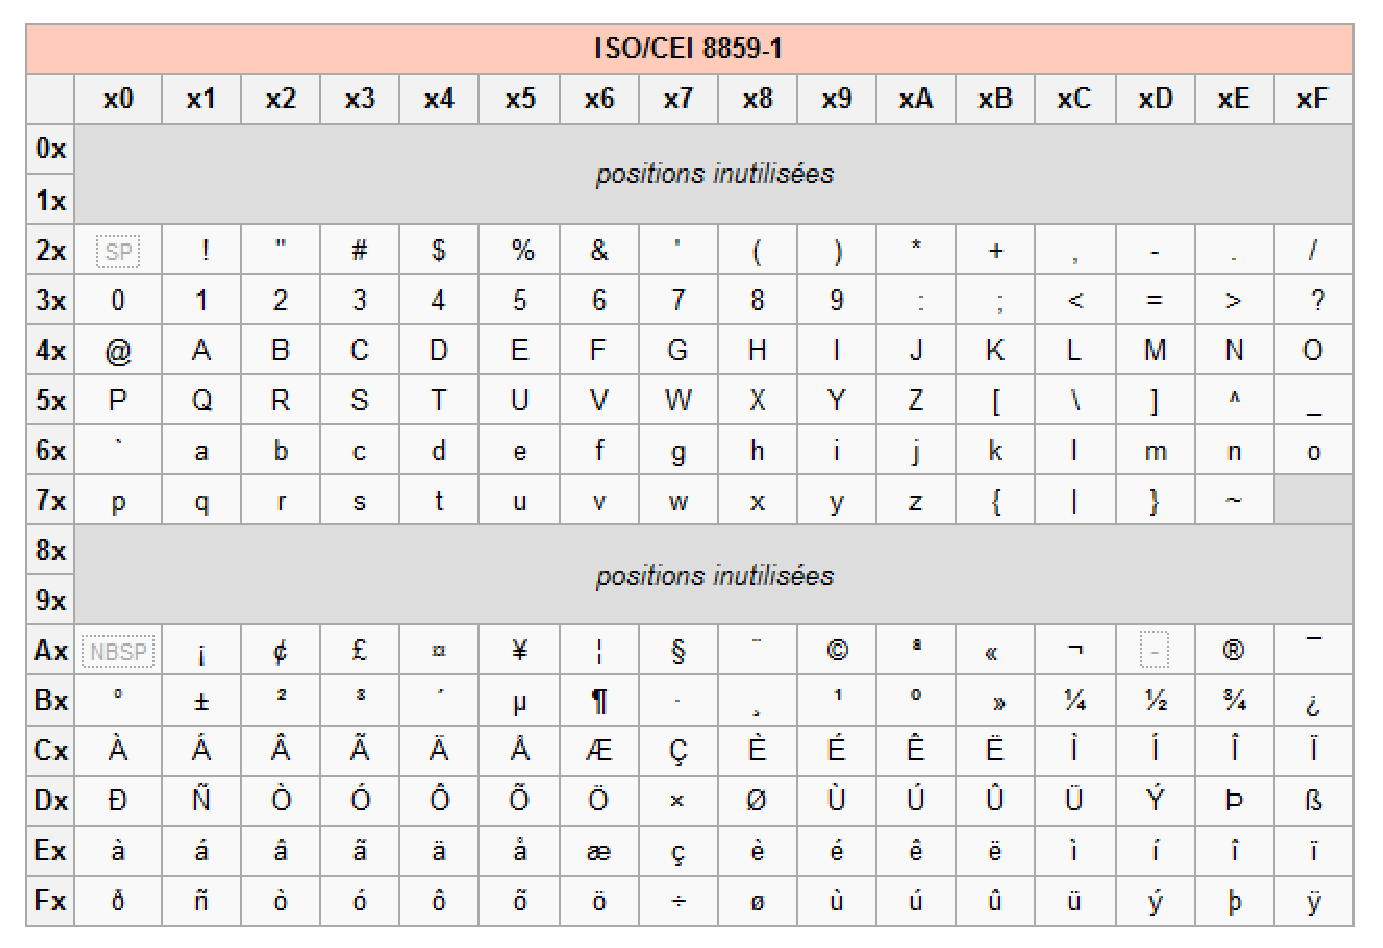
\includegraphics[width=8cm]{tableASCII}
 \label{fig:tableASCII}
\end{figure}

L’encodage universel des caractères est réalisé soit par l’Unicode ou l’UFT-8 (Universal Transformation Format).

Les fichiers de type binaire ne contiennent pas (exclusivement) du texte. Et ils ne peuvent être convenablement traités que par des logiciels spécialisés. Un fichier PDF, une image JPEG ou un mp3 sont quelques exemples de fichiers binaires.

Dans la suite, on n’utilisera que des fichiers de type texte.

%\newpage
\section*{Ouvrir/fermer un fichier}

On peut ouvrir un fichier grâce à la fonction \verb|open('emplacement/nom')| qui permet d'accéder à un fichier stocké dans l'ordinateur, en spécifiant son emplacement sur le disque et son nom. Pour pouvoir manipuler les données du fichier, il faut l'affecter à une variable, comme n'importe quelle autre structure de données. Par exemple, on peut l'affecter à la variable \verb|fichier| :

\begin{minted}[]{python}
fichier = open('emplacement/nom') 
\end{minted}

\begin{enumerate}
\item Aller dans le répertoire « Ressources », puis « PTSI », puis « TP6 ». Copier le fichier {\og}TP6.txt{\fg} et coller le dans votre répertoire personnel situé dans {\og}Dossiers personnels/PTSI{\fg}.\\
Dans votre répertoire personnel, faire un clic-droit sur le fichier. Choisir « propriétés ». Sélectionner et copier le chemin d'accès qui apparaît après « Emplacement ».

\item Dans l'éditeur de script, écrire l'instruction qui ouvre le fichier grâce à la fonction \verb|open| et l'affecter à une variable (par exemple \verb|fichier|). Dans tous les cas, on ferme toujours en fin de procédure le fichier par l'instruction :
\begin{minted}[]{python}
fichier.close() 
\end{minted}

\end{enumerate}

\section*{Traitement caractère par caractère d'un fichier}

Une fois affecté à une variable, un fichier est une structure de données de type \verb|file| qui est itérable et qui peut être parcourue ligne par ligne. De plus, chaque ligne du fichier est une chaîne de caractère (type \verb|str|) qui est elle-même itérable et qui peut être parcourue caractère par caractère. En imbriquant correctement deux boucles itératives on peut donc lire un fichier texte caractère par caractère.

\begin{enumerate}
\setcounter{enumi}{2}
\item Écrire une procédure permettant de parcourir chacun des caractères de chacune des lignes du fichier \verb|TP6.txt| et de les afficher à l'écran.
\end{enumerate}

Attention ! Si vous voulez lire plusieurs fois de suite le même fichier un problème survient : pour python, une fois qu'un fichier a été lu entièrement{\dots} il n'y a plus rien à lire ! On dit que python est positionné en fin de fichier. Pour pallier ce problème, on peut :
\begin{itemize}
 \item fermer le fichier comme il est recommandé de le faire à la fin de chaque procédure ; puis le réouvrir et le réaffecter à une variable si on veut le relire ; 
 \item utiliser la méthode \verb|.seek()| qui permet de positionner python où on veut dans le fichier ; par exemple :\\
 \verb|fihcier.seek(0)| permet de repositionner python en début du fichier \verb|fichier|, comme s'il venait d'être ouvert.
\end{itemize}

%\newpage
On souhaite maintenant récupérer la totalité des données du fichier dans une liste. La liste souhaitée est donc une liste de listes, chaque sous-liste étant une liste des mots d'une ligne. Dans le cas de notre TP, le résultat attendu est donc :
\begin{center}
\verb|[ ['mot1', 'mot2', 'mot3'], ['mot4', 'mot5', 'mot6'], ['mot7', 'mot8', 'mot9'] ]|
\end{center}

Dans le fichier \verb|TP6.txt| chaque mot d'une ligne est séparé par une virgule. On dit qu'un tel fichier est un fichier en « \textit{comma separated values} » (ou csv)\footnote{Un autre type de format très utilisé est le format « \textit{tab separated values} » (ou tsv)  dans lequel chaque mot d'une ligne est séparé par une tabulation.}. D'autre part, pour signifier la fin d'une ligne d'un fichier texte, un caractère spécial (dit caractère d'échappement) est utilisé : \verb|\n|. Cela veut dire que dans le fichier \verb|TP6.txt|, les mots se terminent soit par \verb|','| soit par \verb|'\n'|.

\begin{enumerate}
\setcounter{enumi}{3}
\item À partir du code de la procédure utilisée à la question 3, écrire une procédure permettant de former la liste demandée ci-dessus pour le fichier \verb|TP6.txt|. La logique est la suivante :
\begin{itemize}
 \item on lit les caractères un à un et on forme des mots avec ;
 \item quand un mot est fini, on l'ajoute à la liste des mots d'une ligne ;
 \item quand une ligne est finie, on l'ajoute à la liste des listes des mots de lignes.
\end{itemize}

\item (Uniquement sous Windows.) Quel est le problème rencontré en fin de fichier ? Le résoudre.
\end{enumerate}

\newpage
\section*{Lire, écrire}

Il est possible d'ouvrir un fichier dans plusieurs \textit{modes} : lire (\verb|'r'|), ajouter à la fin (\verb|'a'|), écrire (\verb|'w'|). Les différents modes déterminent le type d'accès aux données (lecture (R) ou écriture (W)) et si les données éventuellement initialement présentes dans le fichier sont effacées à l'ouverture.

\begin{center}
\begin{tabular}{|c|c|c|c|c|}\hline
mode & accès  & réinitialisation & remarque \\\hline
r    & R      & non              & le fichier doit exister \\\hline
r+   & R/W    & non              & le fichier doit exister \\\hline
a    & W      & non              & le fichier doit exister \\\hline
a+   & W/R    & non              & le fichier est créé s'il n'existe pas \\\hline
w    & W      & oui              & le fichier est créé s'il n'existe pas \\\hline
w+   & W/R    & oui              & le fichier est créé s'il n'existe pas \\\hline
\end{tabular}
\end{center}

Par défaut, si on ne précise aucun mode (comme à la section I), c'est le mode \verb|'r'| qui est utilisé. 

Par exemple, pour ouvrir un fichier en lecture/écriture sans réinitialiser le fichier on utilise :
\begin{minted}[]{python}
open('emplacement/nom','r+') 
\end{minted}

Par exemple, pour ouvrir un fichier en écriture uniquement en réinitialisant le fichier on utilise :
\begin{minted}[]{python}
open('emplacement/nom','w') 
\end{minted}

\textbf{On évite absolument d'ouvrir en écriture un fichier qui contient des données que l'on souhaite conserver\footnote{Comme les fichiers données initiales de ce TP par exemple\dots}.}

Pour écrire une chaîne de caractère dans le fichier on peut utiliser la méthode \verb|.write| :\\
\verb|fichier.write(s)| écrit la chaîne de caractères \verb|s| dans le fichier \verb|fichier|.

\begin{enumerate}
\setcounter{enumi}{5}
 \item À partir du code de la procédure utilisée à la question précédente, écrire une procédure permettant de réécrire un nouveau fichier nommé « TP6tab.txt » dans lequel toutes les virgules sont remplacées par des tabulations. (Les tabulations sont codées par le caractère spécial \verb|\t|.)
\end{enumerate}

\section*{Utilisation des méthodes Python}

La lecture itérative caractère par caractère de la section II peut avantageusement être remplacée par les méthodes python associées aux fichiers. Les principales méthodes de la classe \verb|file| sont :
\begin{itemize}
\item \verb|.read()| retourne tout le fichier comme une chaîne de caractères,
\item \verb|.read(n)| retourne une chaîne de caractère d’au moins n octets,
\item \verb|.readline()| retourne une ligne (la ligne courante),
\item \verb|.readlines()| retourne la liste de toutes les lignes du fichier,
\item \verb|.write(s)| écrit la chaîne de caractères \verb|s| dans le fichier (à la position courante),
\item \verb|.writelines(lines)| écrit la ligne (liste de chaînes de caractères) \verb|lines| dans le fichier (à la position courante),
\item \verb|.close()| ferme le fichier,
\item \verb|.next()| retourne la ligne suivante,
\item \verb|.seek(0)| repositionne la lecture/écriture au début du fichier.
\end{itemize}

D'autre part, certaines méthodes de la classe \verb|str| sont très utiles quand on manipule les données d'un fichiers :
\begin{itemize}
\item \verb|.strip()| élimine tous les espaces et caractères d'échappement qui commencent ou terminent une ligne (le marqueur de fin de ligne \verb|'\n'| notamment),
\item \verb|.split(separateur)| retourne une liste des séquences de caractères qui dans la chaîne de caractères sont séparées par \verb|separateur|,
\item \verb|.replace(ancienne, nouvelle)| renvoie une copie de la chaîne de caractère dans laquelle \verb|chaine| la suite de caractères \verb|ancienne| par \verb|nouvelle|.
\end{itemize}

\begin{enumerate}
\setcounter{enumi}{6}
 \item Refaire les questions 4 et 6 à l'aide de méthodes python.
 \item Écrire à l'aide de méthodes python une procédure permettant de copier le contenu du fichier \verb|TP6tab.txt| dans un nouveau fichier nommé « TP6.tsv ».
\end{enumerate}

%\newpage
\section*{Exercice}

Le fichier \verb|notes.csv| est situé dans le même répertoire que \verb|TP6.txt| et contient le bulletin scolaire de quinze élèves avec, sur chaque ligne, séparés par des virgules : leur nom, leur prénom et trois notes (écrites avec un séparateur décimal anglo-saxon, c'est-à-dire un point). Les coefficients de chacune des notes sont (dans l'ordre) 1, 2 et 3. On souhaite modifier le fichier pour rajouter une colonne supplémentaire dans laquelle figure la moyenne de chaque élève et rajouter une ligne d'en-têtes pour que le fichier soit plus explicite.

\begin{enumerate}
\setcounter{enumi}{8}

\item Copier/coller le fichier \verb|notes.csv| dans votre répertoire personnel.

\item Écrire une procédure qui :

\begin{itemize}
 \item récupère les données présentes dans le fichier,
 \item calcule la moyenne de chaque élève,
 \item calcule la moyenne des moyennes de la classe et l'écart-type des moyennes de la classe,
 \item crée un nouveau fichier \verb|notes_et_moyennes.csv|, dont le contenu est celui du fichier \verb|notes.csv| avec :
 \begin{itemize}
  \item une ligne supplémentaire de commentaire en en-tête de fichier décrivant les différentes colonnes (nom, prénom,notes1,notes2,notes3,moyenne),
  \item ajoute la moyenne de chaque élève en fin de ligne,
  \item calcule la moyenne globale et l'écart-type des moyennes de la classe et les affiche à l'écran.
 \end{itemize}

\end{itemize}
\end{enumerate}

Pour le calcul de l'écart-type, on doit importer la fonction racine carrée qui n'est pas présente dans les bibliothèques du cœur de python mais est présente dans la bibliothèque \texttt{math}. En début de script, juste avant les premières instructions, on insère :

\begin{minted}[]{python}
import math as math
\end{minted}

Ce qui permet d'utiliser ensuite la fonction racine carrée dont la syntaxe est :\\
\texttt{math.sqrt(nombre)}

% version numpy cf TP6 2014-2015
% Pour le calcul des moyennes et de l'écart-type des moyennes, on pourra avantageusement tirer profit des fonctionnalités des tableaux numpy, en faisant attention :
% \begin{itemize}
%  \item au fait qu'un tableau numpy ne peut contenir qu'un seul type de données (par exemple chaîne de caractère ou flottant mais pas les deux) ;
%  \item au fait que tout ce qui est lu dans un fichier est sous forme de chaîne de caractères ; il faut donc prévoir des conversions de types avant de mener les calculs numériques.
% \end{itemize}
% 
% Quelques fonctionnalités des tableaux numpy, sur l'exemple d'un tableau à deux dimensions s'appelant \verb|tableau|:
% \begin{itemize}
%  \item Appel de la ligne i : \verb|tableau[i]|
%  \item Appel de la colonne j : \verb|tableau[:,j]|
%  \item Appel de toutes les lignes entre la deuxième et la dernière \verb|tableau[1:]|
%  \item Appel de toutes les lignes entre la deuxième et l'avant-dernière \verb|tableau[1:len(tableau-1)]|
%  \item Appel des lignes entre la quatrième et la dixième incluses : \verb|tableau[3:11]|
%  \item Appel des colonnes entre la quatrième et la dixième incluses : \verb|tableau[:,3:11]|
%  \item Obtenir les dimensions du tableau : \verb|np.shape(tableau)|
%  \item Obtenir le nombre de lignes du tableau : \verb|np.shape(tableau)[0]|
%  \item Obtenir le nombre de lignes du tableau : \verb|np.shape(tableau)[1]|
% \end{itemize}

\end{document}
